\chapter{Theoretical background} \label{chap_theoreticalbackground} 

The goal of this thesis is to investigate whether \gls{ca} approach aligns with the goals
of \gls{ns}. Therefore, it is essential to have a comprehensive understanding of software
stability and the key concepts, principles, and architectures that impact software
stability.

This chapter begins by examining the concepts of software stability, evolvability, and
modularity, highlighting their significance in achieving software stability in \gls{ns}.
This is followed by a brief overview of the design theorems and proposed architecture of
\gls{ns}.

The subsequent sections of the thesis explore the fundamental principles that underlie
\gls{ca}, as well as its proposed architectural designs. Finally, the thesis
concludes by discussing which aspects of \gls{ca} align with the principles of
\gls{ns} and contribute to achieving software stability in this approach.

\section{Normalized Systems: Impacting software stability} \label{sec:ns_theory}

\gls{ns} is a software development approach that prioritizes achieving software stability
through the use of standardized, modular components and interfaces. This theory is
informed by several scientific disciplines, including systems theory, mathematics, and
computer science, as well as some other software development approaches, such as agile
development and domain-driven design.

\gls{ns} originated in the field of software engineering. However, the underlying theory
of \gls{ns} can be applied to various other domains, such as Enterprise Engineering,
Business Process Modeling, and document management. This research acknowledges the
software engineering background of \gls{ns}. It consistently refers to software and
Information Systems when referring to \enquote*{artifacts.} However, the reader should
realize that the concepts and artifacts are not restricted to software artifacts alone.
\subsection{Towards stability} \label{subsec:on_stability}

In several disciplines, stability has been defined as \emph{Bounded Input Bounded Output}
(BIBO). It is the fundamental property of a system when subjected to bounded input
disturbances. BIBO stability ensures that the output of a system will also be bounded,
preventing uncontrolled or unexpected behavior \parencite[270]{mannaert_normalized_2016}. 

A real-world example of the importance of stability is the Tacoma Narrows Bridge in
Washington State, USA. This bridge, depicted in Figure \ref*{fig:bridge}, collapsed on
November the 7th, 1940. This was caused due to wind-induced oscillations called
aeroelastic flutter. The wind (Input) induced oscillations in the bridge, causing it to
start swaying back and forth (Output). These oscillations were initially small, but as
they continued, they began to increase in amplitude and magnitude. Eventually, this 
caused the bridge to collapse.

\begin{figure}[H]
    \centering
    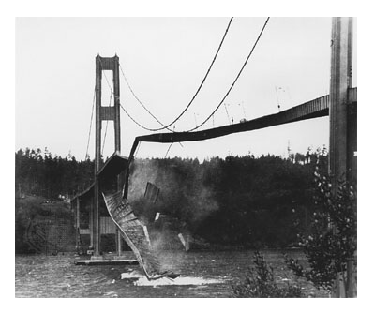
\includegraphics[width=0.6\textwidth]{Figures/bridge.pdf}
    \caption[TNB]{Tacoma Narrows Bridge (Galloping Gertie)}
    \label{fig:bridge}
\end{figure}

Stability can also be used in the context of software engineering. In the context of
\gls{ns}, it is considered a critical property that ensures that the software is not
excessively sensitive to small changes \parencite[270]{mannaert_normalized_2016}. New
functional requirements should only lead to a fixed and expected amount of changes in
the source code. 

Conversely, instabilities occur when the total number of modifications relies on the size
of the software artifact. When there are software instabilities, the number of changes
will grow over time in parallel with the growth of the system. These instabilities are
referred to as combinatorial effects \parencite[270]{mannaert_normalized_2016}. 

When combinatorial effects are absent, the software artifact can be considered evolvable.
\subsection{Towards Evolvability} \label{sec:on_evolvability}

In \gls{ns} Evolvability is a crucial property in order to achieve stable software
systems. An evolvable system can adapt over time in response to changing requirements.
\gls{ns} attempts to achieve evolvability by providing guidelines, principles and theorems
n order to achieve a modular (and scalable) architecture that allows for easy
adaptability, extensibility and the replacement of components with a minimum impact on the
quality of the functionality, and the overall structures of the architecture. This is
achieved through the use of formalized models that define the system's components,
interfaces, and behavior, as well as through the separation of concerns between different
parts of the system.

There are several aspects concerning the evolvability of software systems. One of which is
the modularity of the architecture. There is also a wide consensus about two fundamental
rules when thinking of-, and designing modularity: \emph{high cohesion} and \emph{low
coupling} \autocite[22]{mannaert_normalized_2016}.
\subsection{Modularity}

A Software module can be defined as self-contained units of code that perform specific
tasks or sets of tasks within a larger system. A software module is designed to operate
independently of other modules, with well-defined interfaces that allow it to communicate
and exchange data with other modules if necessary \autocite[22]{mannaert_normalized_2016}.

A module can be considered a hierarchical and recursive concept. They are independent of
their size (lines of code) or computational magnitude. They can be as small as a function
as part of a class. The class itself can also be considered a module. A group of classes
contained in a Dynamic Link Library (DLL) or Application Programming Interface (API) can
also be considered a module of an even bigger system. 

An important part of the design of a software system is to identify the possible different
modules and their interaction interfaces. Figure \ref{fig:modulair_components} presents a
high-level depiction of modular manifestations in the artifact, with additional examples
of modularity found in more granular implementations. Further discussion of this
architecture is provided in Chapter \ref{sec:ca_theory}.
\subsection{Cohesion} \label{subsubsec_on_cohesion}

The term cohesion denotes the extent to which the various structural components of a
software system operate cohesively towards a singular and well-defined objective or goal.
Empirical studies in software engineering have extensively demonstrated the significance
of cohesion, linking higher levels of cohesion with reduced defects, enhanced
maintainability, and greater openness to change. Consequently, achieving high cohesion has
been associated with an overall improvement in software quality attributes such as
reliability, maintainability, reusability, and evolvability.

Cohesion facilitates the reduction of complexity and interdependence among the components
of a system, thereby contributing to a more efficient, maintainable, and reliable system.
By organizing components around a shared purpose or function or by standardizing their
interfaces, data structures, and protocols, cohesion can offer the following benefits:

\begin{itemize}
    \item \textbf{Reduce redundancy and duplication of effort}: \\
    Cohesion ensures that components are arranged around a common purpose or function,
    reducing duplicates or redundant code. This simplifies system comprehension,
    maintenance, and modification.
    \item \textbf{Promoting code reuse:}\\
    Cohesion facilitates code reuse by making it easier to extract and reuse components
    designed for specific functions. This saves time and effort during development and
    enhances overall system quality.
    \item \textbf{Enhance maintainability:}\\
    Cohesion decreases the complexity and interdependence of system components, making it
    easier to identify and rectify bugs or errors in the code. This improves system
    maintainability and reduces the risk of introducing new errors during maintenance.
    \item \textbf{Increase scalability:}\\
    Cohesion improves a system's scalability by enabling it to be extended or modified
    effortlessly to accommodate changing requirements or conditions. By designing
    well-organized and well-defined components, developers can easily add or modify
    functionality as needed without disrupting the rest of the system.  
\end{itemize}


\subsection{Coupling} \label{subsec:on_coupling}

Coupling is an essential concept in software engineering that pertains to the degree of
interdependence among software modules and components. The level of coupling between
modules denotes the strength of their relationship, whereby a high level of coupling
implies a significant degree of interdependence. Conversely, low coupling signifies a
weaker relationship between modules, where modifications in one module are less likely to
impact others. Although not always possible, the level of coupling between the various
modules of the system should be kept to a bare minimum.

The negative impact of excessive coupling on software systems is considerable. High
coupling can render software systems challenging to maintain, modify, or evolve. It can make
it considerably more challenging to find the root cause of potential bugs. Additionally, it
causes fragility in the system, where slight modifications in one module can trigger
cascading failures throughout the entire system. Therefore, it is crucial for software
engineers to minimize coupling between modules while maintaining a cohesive design. By
developing systems with low coupling, software engineers can construct more maintainable,
scalable, and adaptable systems that are easier to evolve.

Coupling in software engineering can take several forms, including content, common,
control, stamp, and data coupling. Content coupling occurs when one module accesses or
modifies the internal data or logic of another module, leading to high interdependence and
difficulty in isolating errors. Common coupling occurs when several modules access and use
the same global data, increasing their interdependence and reducing modularity. Control
coupling occurs when one module controls the execution flow of another module, making it
challenging to modify or reuse the controlled module. Stamp coupling arises when two modules
share a common data structure, leading to tight coupling and high interdependence.
Finally, data coupling exists when two modules share data, which can lead to coupling
between them.

One attempt to lower coupling in the expanded artifact is to prefer stamp coupling over
data coupling through the API interface. This is done by making use of RequestModels and
ViewModels, instead of the actual data element (see example in Listings \ref{SnipModelExamples}).
Depending on the use case, only the required data is passed down to the view, or in the
case of a command accepted as an input parameter.

\lstinputlisting[
    caption={The ViewModel \parencite{koks_componentviewmodel_2023} and RequestModel
    \parencite{koks_deletecomponentcommand_2023} of the Entity 'Component'
    \parencite{koks_component_2023}},
    label={SnipModelExamples}]
    {Snippets/ModelExamples.cs}
\subsection{Expansion and code generation} \label{subsec:expansion}

Creating and maintaining a stable and evolvable system is a particularly difficult and
meticulous engineering job. Developers are required to have a sound knowledge of \gls{ns},
whilst implementing new requirements in an always consistent manner. Given the required
recurring structure, it can be perceived as a repetitive and therefore boring taks.
\parencite[219]{mannaert_normalized_2016}. On top of that, rejecting the temptation to
take shortcuts in order to follow the business's time-to-market requirements.

Given the above, it is quite logical to automate the instantiation process of software
structures and use code generation for recurring
tasks\parencite[403]{mannaert_normalized_2016}. This is where code expansion comes in
place. The concept of code expansion does not only refer to the automatic process of
adapting and maintaining software to new requirements, architectural enablers and/or
technological alterations. It also embraces manually added craftings to the software, the
so-called plugin code. These craftings are preserved after each expansion by a method that
is called harvesting and rejuvenation \parencite[405-406]{mannaert_normalized_2016}.


\subsection{The Theoretical Framework} \label{subsec:ns_desing_theorems}

\gls{ns} consists of a theoretical framework describing a set of design principles. These
principles are the basis for achieving the concepts of stability, evolvability, and
modularity. \gls{ns} provides a rigorous and mathematical foundation for these theorems
and they offer guidelines for designing and developing software systems. In the following
sections, we will focus on the principles of \gls{ns} very briefly as they have been
extensively described in various scientific papers.

We know from Chapter \ref{sec:artifact_requirements} that the design artifacts, as a part
of this research, are implemented based on the \gls{ca} principles. Therefore, contrary to
Chapter \ref{sec:ca_theory}, there will be no references to the manifestations of the NS
design theorems in the design.
\subsubsection*{Separation of Concerns}

\gls{soc} as a principle has first been mentioned by
\citeauthor{dijkstra_selected_1982}\footnote{\url{https://en.wikipedia.org/wiki/Separation_of_concerns}}
as the crucial principle to design modular software architecture
\parencite[]{dijkstra_selected_1982}. \gls{soc} promotes the idea that a program should be
divided into distinct sections, each addressing a separate concern or aspect of a design
problem. This allows for a more organized and maintainable source code. When implemented
correctly, a change to one concern does not affect the others. \gls{soc} should be applied
at the level of individual modules, rather than the level of an entire program.

\gls{soc} has been adopted as one of the design theorems of \gls{ns}, although it has a
stricter definition of this principle\parencite{mannaert_normalized_2016}.

\begin{tcolorbox}[boxrule=0.1pt, colback=mygray, title=Theorem I,colbacktitle=gray]
    \textit{A processing function can only contain a single task to achieve stability.}
\end{tcolorbox}
\subsubsection*{Data version Transparancy}

\gls{dvt} is the act of encapsulation of data entities for specific tasks at hand. This
results in the fact that data structures can have multiple versions often mentioned as
Data Transfer Objects in modern software engineering projects. In other words, it should
be possible to update the data entity without affecting the processing functions. This
leads to the following description of the theorem \parencite[280]{mannaert_normalized_2016}.

\mycolorbox{A data structure that is passed through the interface of a processing function
needs to exhibit version transparency in order to achieve stability.}{Theorem II}

\gls{dvt} is widely used in various technological applications. practically every web
service currently known supports some type of versioning. In restful APIs for example, it
is common practice to support versioning over the URI. It is considered a best practice
to encapsulate breaking changes in a new version of the endpoint/service so that the
consumers are not (directly) affected by the change. In modern Object Oriented languages,
gls{dtv} is also supported by the ability to determine the scope of visibility of the
modifiers of the various programming constructs like fields, properties, interfaces and
classes. Also known as information hiding
\parencites{parnas_criteria_1972}[278]{mannaert_normalized_2016}.
\subsubsection*{Action version Transparancy}
\gls{avt} is the property of a system to modify existing processing functions without
affecting the existing ones. It should be possible to upgrade a function without affecting
the callers of those functions. This description leads to the following theorem
\parencite[282]{mannaert_normalized_2016}.

\begin{tcolorbox}[boxrule=0.1pt, colback=mygray, title=Theorem III,colbacktitle=gray]
    \textit{A processing function that is called by another processing function, needs to exhibit version transparency in order to achieve stability.}
\end{tcolorbox}

Most of the modern technology environments support some form of \gls{avt}. Polymorphism is
a widely used technique in order to support this theorem. Specifically, parametric
polymorphism \footnote{\url{https://en.wikipedia.org/wiki/Parametric_polymorphism}} allows
for a processing function to have multiple input parameters. There are also quite some
design patterns supporting this theorem. Some random examples are the state pattern
\footnote{\url{https://en.wikipedia.org/wiki/State_pattern}}, facade pattern
\footnote{\url{https://en.wikipedia.org/wiki/Facade_pattern}} and observer pattern
\footnote{\url{https://en.wikipedia.org/wiki/Observer_pattern}}.
\subsubsection{Separation of State}

\gls{sos} is a theorem that is based on the idea that processing functions should not
contain any state information but instead should rely on external data structures to store
state information. By separating state information from processing functions, Normalized
Systems can achieve a higher level of flexibility and adaptability. External data
structures can be updated or replaced without affecting the processing functions
themselves, which greatly reduces the change of unwanted ripple effects. This theorem is
described as followed: \parencite[258]{mannaert_normalized_2016}.

\mycolorbox{Calling a processing function within another processing function, needs to exhibit state keeping in order to achieve stability.}{Theorem IV}
\subsection{Normalized Elements} \label{subsec_ns_elements} 

In the context of the \ns Theory approach, the goal is to design evolvable software,
independent of the underlying technology. Nevertheless, when implementing the software and
its components, a particular technology must be chosen. For Object Oriented Programming
Languages like Java, the following Normalized Elements have been proposed
\parencite{mannaert_normalized_2016}[363-398].

This research's artifacts utilized C\# as the primary programming language. It is essential
to recognize that different programming languages may necessitate alternative constructs
\parencite{mannaert_normalized_2016}[364]. Given the strong similarities between C\# .NET
and Java, it is assumed that the same Normalized Elements are applicable for C\# .NET
implementation of this research's artifacts.

\subsubsection{The Data Element}
This is an object that represents a piece of data in the system. Data elements are used to
pass information between processing functions and other objects. In \ns,
data elements are typically standardized to ensure consistency across the system.

\subsubsection{The Task Element}
This is an object that represents a specific task or action in the system. Tasks can be
composed of one or more processing functions and can be used to represent complex
operations within the system.

\subsubsection{The Connector Element}
This object is used to connect different parts of the system. Connectors can be
used to link processing functions, data elements, and other objects, allowing them to work
together seamlessly.

\subsubsection{The Flow Element}
This object represents the flow of control through the system. It determines the order in
which processing functions are executed and can be used to handle error conditions or
other exceptional cases.

\subsubsection{The Trigger Element}
a trigger element is an object that reacts to specific events or changes in the system
by executing predefined actions.

\section{Clean architecture: A design philosophy}\label{sec_ca_theory}

\gls{ca} is a software design philosophy that emphasizes the organization of code
into independent, modular layers with distinct responsibilities. This approach aims to
create more flexible, maintainable, and testable software systems by enforcing the
separation of concerns and minimizing dependencies between components. The goal of clean
architecture is to provide a solid foundation for software development, allowing
developers to build applications that can adapt to changing requirements, scale
effectively, and remain resilient against the introduction of bugs
\parencite{robert_c_martin_clean_2018}.
\subsection{The Design principles} \label{subsec_design_principles}

\Citeauthor{robert_c_martin_clean_2018} argues that, without a solid (pun intended) set of
design principles a design and architecture can quickly turn into a well-intended mess
of bricks and building blocks. This is where the SOLID design principles come into place.

SOLID is an acronym for \gls{solid}. The \gls{solid} principles guide the developer on how
to arrange the architecture of the software system. It can be considered a set set of
rules on how to arrange data structures and functions into classes
\parencite[78]{robert_c_martin_clean_2018}.

The upcoming sections will provide a brief overview of each of the SOLID principles, as
there is a plethora of literature on this subject. In chapter
\ref{sec_artifact_requirements} we learn that one of the requirements is to design the
artifact solely based on the design approach of \ca. As such, each principle's description
will be accompanied by one or more manifestation examples in the artifact, aligning with
the research objectives.
\subsubsection{The Single Responsibility Principle} \label{subsubsec:srp}

The \gls{srp} is one of the fundamental design principles of \gls{ca}. The principle
advocates designing systems with high cohesion and low coupling. The \gls{srp} states that
each module in a system should have only one reason to change. That is, it should have a
single responsibility. No matter the granularity of the module, so implementations of
methods, classes, libraries and architecture layers should adhere to \gls{srp}. By
adhering to the principle, each module becomes highly cohesive, meaning that its
responsibilities are closely related and well-defined, while also being decoupled from
other modules \parencite[81]{robert_c_martin_clean_2018}.

The final statement of \gls{srp} is as followed
\parencite[82]{robert_c_martin_clean_2018}.

\mycolorbox{A module should	be responsible to one, and only one, actor.}{\acrlong{srp}}

\gls{srp} is closely related to the concept of \gls{soc}, which also advocates separating
a system into distinct parts. Although not that clearly stated in the literature,
\citeauthor{robert_c_martin_clean_2018} argues that \gls{soc} intends to have a separation
on a functional level and architectural level. This divides a system into different layers
or components based on their functional roles. \gls{srp} is concerned with separating the
responsibilities of individual modules regardless of the granularity of the module.
\parencite[205]{robert_c_martin_clean_2018}.With this in mind, \gls{srp} adheres more to
the definition of \gls{soc} from \gls{ns}. \textit{A processing function can only contain
a single task to achieve stability.} (see chapter \ref{subsubsec:soc}
\nameref{subsubsec:soc}).

There are various manifestations of \gls{srp} implemented in the artifacts. One of which is
already mentioned in Figure \ref{fig:modulair_components}, where \gls{srp} is applied to
separate the domain logic from the application, infrastructure and presentation logic. One
could argue that this manifestation is more related to \gls{soc}, considering the high
granularity of the components.

A better example is the separation of handlers that are part of the Clean Architecture
Expander. Each of those handlers executes an isolated part of the expanding process.
Consider the Listing \ref{SipEntityExpander} \nameref{SipEntityExpander}
\parencite{koks_expandentitieshandlerinteractor_2023} for example. This Handler is solely
responsible for the generation of data entities. 

\begin{figure}[H]
    \centering
    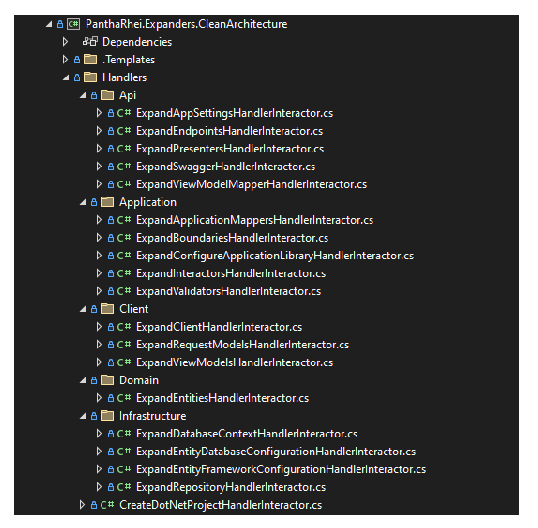
\includegraphics[width=0.6\textwidth]{Figures/expander_handlers.pdf}
    \caption[handlers]{Each of the handlers handles an isolated part of the expanding process.}
    \label{fig:handlers}
\end{figure}

\lstinputlisting[
    caption={The \citetitle{koks_expandentitieshandlerinteractor_2023}},
    label={SipEntityExpander}]
    {Snippets/ExpandEntitiesHandlerInteractor.cs}
\subsubsection*{The Open-Closed Principle} \label{subsubsec:ocp}

The \gls{ocp} was first mentioned by \Citeauthor{meyer_object-oriented_1997}. He described
the principle as followed \parencite[79]{meyer_object-oriented_1997}. The reference here
is for the second edition of the book, the original version is from 1988.

\mycolorbox{A module should	be open for extension but closed for modification.}{\acrlong{ocp}}

\gls{ocp} emphasizes the importance of designing systems that are open for extension but
closed for modification. This means that the behavior of implementations can be extended
without modifying its source code. The OCP promotes the use of abstraction and
polymorphism to achieve this goal. By using interfaces, and abstract classes a system can
be designed to allow for new behaviors to be added through extension, without changing the
existing code. The OCP is one of the driving forces	behind the architecture	of systems.
The goal is	to make	the	system easy	to extend without incurring a high impact of change
\parencite[94]{robert_c_martin_clean_2018}.

A relevant manifestation of \gls{ocp} are all the different implementations of expander
handlers in figure \ref{fig:handlers}. The availability of the
\code{koks_iexpanderhandlerinteractor_2023} interface makes it possible to add more
functionality to the CleanArchtictureExpander without modifying any existing
implementation. New handlers are added by extension, and when implemented correctly, the
handler is automatically executed in the desired order and the required conditions.

\lstinputlisting[
    caption={The \citetitle{koks_iexpanderhandlerinteractor_2023}},
    label={SipIExpanderHandlerInteractor} ]
    {Snippets/IExpanderHandlerInteractor.cs}

\lstinputlisting[
    caption={The \citetitle{koks_iexecutioninteractor_2023}},
    label={SipIExecutionInteractor} ]
    {Snippets/IExecutionInteractor.cs}

The fact that \citecode{koks_iexpanderhandlerinteractor_2023} derives from
\citecode{koks_iexecutioninteractor_2023} is another manifestation of \gls{ocp}. This
design decision allows for object types that need to be treated as executables by the
\code{koks_codegeneratorinteractor_2023}. Examples are
\citecode{koks_regionharvesterinteractor_2023},
\citecode{koks_regionrejuvenatorinteractor_2023},
\citecode{koks_preprocessorinteractor_2023} and
\citecode{koks_postprocessorinteractor_2023}. 

Listing \ref{SipCodeGeneratorInteractor} shows the
\code{koks_codegeneratorinteractor_2023} that cohesively executes all of the
\code{koks_iexecutioninteractor_2023} in order. The software engineer only has to focus on
implementing the specific type of \code{koks_iexecutioninteractor_2023} without having to
affect the implementation. This is by definition an example of \enquote{open for
extension} and \enquote{closed for modifications}.


\lstinputlisting[
    caption={The \citetitle{koks_codegeneratorinteractor_2023}},
    label={SipCodeGeneratorInteractor} ]
    {Snippets/CodeGeneratorInteractor.cs}
\subsubsection{The Liskov Substitution Principle} \label{subsubsec:lsp}


The \gls{lsp} is a fundamental concept in object-oriented programming that deals with the
behavior of derived objects (aka sub-types). The principal is named after Barbara Liskov
who first introduced the principle in a paper she co-authored in 1987. Barbara Liskov
wrote the following statement as a way of defining subtypes
\parencite[95]{robert_c_martin_clean_2018}.

\mycolorbox{If for each	object o1 of type S there is an	object o2 of type T such that for
all programs P defined in terms of T, the behavior of P	is unchanged when o1 is
substituted for	o2 then S is a subtype of T.1}{\acrlong{lsp}}

In simpler terms: If you have an object \textit{Volvo} of type \textit{Vehical}, it should be
possible to substitute it for an object \textit{Toyota} of type \textit{Vehical} in any
program that was defined in terms of \textit{Vehical}, without affecting the program's
correctness. This applies to all programs, not just a specific one.

The principle is based on the idea that a subtype should be semantically substitutable for
its base type. This means that the subtype should behave in a way that is consistent with
the expectations of the base type and should not introduce any new behaviors or violate
any of the constraints imposed by the base type.

The practical implications of \gls{lsp} are many. In software design, it means that we
should strive to create subtypes that are as similar as possible to their base types in
terms of their behavior and the constraints they impose. In testing, it means that we
should test subtypes to ensure that they behave correctly when used in place of their base
types.

Consider \citecode{koks_abstractexpander_2023}. This (abstract) object type allows for
multiple implementations of \textit{Expanders}. The main example is the
\citecode{koks_cleanarchitectureexpander_2023} which is responsible for generating the
expanded artifact that is part of this research. Different types of expanders could be
added to the generator, ensuring they all behave in the same way.

The \citecode{koks_icreategateway_2023} in Listing \ref{SipICreateGateway} is another
example. The artifact has two implementations of this interface. The data of the entities
are currently stored in the database, but harvest data is serialized to XML using the same
\code{koks_icreategateway_2023} interface. With this design decision, it is very easy to adapt
to a different type of storage mechanism if future requirement demand such a change.

One might notice the similarities with the \gls{ocp}. The difference is that the \gls{ocp}
focuses on the extensibility of the system, without having to modify existing code.
\gls{lsp} ensures that the behavior of different subtypes is following the required
functionality. \gls{lsp} supports \gls{ocp}, but it is not the only way of doing so.

\lstinputlisting[
    caption={The \citetitle{koks_icreategateway_2023}},
    label={SipICreateGateway} ]
    {Snippets/ICreateGateway.cs}

\lstinputlisting[
    caption={The \citetitle{koks_genericrepository_2023} and \citetitle{koks_harvestrepository_2023}},
    label={SipICreateGatewayImplementations} ]
    {Snippets/ICreateGatewayImplementations.cs}


\subsubsection*{The Interface Segregation Principle} \label{subsubsec:isp}

The \gls{isp} suggests that software components should have narrow, specific interfaces
rather than broad, general-purpose ones. The \gls{isp} states that no client code should
be forced to depend on methods it does not use. In other words, interfaces should be
designed to be as small and focused as possible, containing only the methods that are
relevant to the clients that use them. This allows clients to use only the methods they
need, without being forced to implement or depend on unnecessary methods
\parencite[104]{robert_c_martin_clean_2018}.

Overall, the \gls{isp} is about designing interfaces that are tailored to the specific
needs of the clients that use them, rather than trying to create one-size-fits-all
interfaces that may be bloated or unwieldy.

Take a look at Listing \ref{SipISPExample}. In order to comply with the \gls{isp} the
design decision was made to separate all \gls{crud} operations into separate interfaces.
In the example of the \citecode{koks_appseederinteractor_2023} (see \ref{SipISPExample})
only the delete and create gateways where required. An alternative approach was to create
an IGateway interface containing all of the \gls{crud} operations. Following this approach
would lead to dependencies to all \gls{crud} operations in the
\code{koks_appseederinteractor_2023}.

\lstinputlisting[
    caption={The Gateways for Create, Read, Update, Delete operations},
    label={SipISPExample}]
    {Snippets/ISP_Example.cs}
\subsubsection{The Dependency Inversion Principle} \label{subsubsec_dip} \todo{explain
how dependency injection can benefit the implementation and align with \ref{tab_convergence_dip}}

The \gls{dip} prescribes that high-level modules should not depend on low-level modules,
and that both should depend on abstractions. The principle emphasizes that the
architecture should be designed in such a way that the flow of control between the
different objects, layers and components are always from higher-level implementations
to lower-level details.

In other words, high-level implementations like business rules, should not be concerned
about low-level implementations, such as the way the data is stored or presented to the
end user. Additionally, both the high-level and low-level implementations should only
depend on abstractions or interfaces that define a contract for how they should interact
with each other \parencite[109]{robert_c_martin_clean_2018}.

This approach allows for great flexibility and a modular architecture. Modifications in
the low-level implementations will not affect the high-level implementations as long as
they still adhere to the contract defined by the abstractions and interfaces.
Similarly, changes to the high-level modules will not affect the low-level modules as long
as they still fulfill the contract. This reduces coupling and ensures the evolvability
system over time, as changes can be made to specific modules without affecting the rest of
the system.

Manifestations in the artifacts are ample. One of which is the consistent use of the
Dependency Injection pattern. In order to prevent the risks of displacing and dispersing
dependencies all over the system \parencite[214]{mannaert_normalized_2016} we are using
dependency containers. Each module is maintaining its own dependencies, which are
bootstrapped at application startup (see Listing \ref{list_dip})
\parencite{koks_generator_2023}.

\lstinputlisting[
    caption={Bootstrapping the dependencies of each component/layer of the
    generator artifact.},
    label={list_dip}]
    {Snippets/Dip.cs}

A more abstract example is the separation of required modules into separate component
libraries. This applies to both the generated and generator artifact (see Figure
\ref{fig_solutions}). The actual compliance to the \gls{dip} is how the flow of control
between the components is organized. This is accurately depicted in Figure
\ref{fig_modulair_components} \nameref{fig_modulair_components}.

\begin{figure}[H]
    \centering
    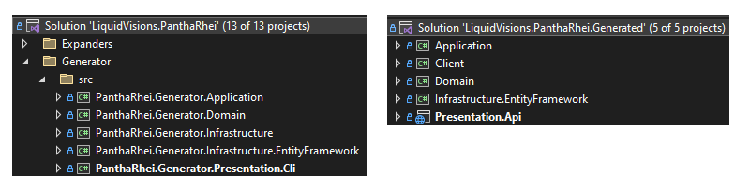
\includegraphics[width=1\textwidth]{Figures/solutions.pdf}
    \caption[modularity]{Separation of component libraries.}
    \label{fig_solutions}
\end{figure}
\subsection{Layers and components} \label{subsec:layers}

Clean architecture organizes software systems into distinct layers or components, each
with its own responsibilities. This structure promotes the separation of concerns,
maintainability, testability, and adaptability. The following section is a short
description of each of the layers \parencite{robert_c_martin_clean_2018}.

\subsubsection*{Domain layer}
This layer contains the core business objects, rules, and domain logic of the application.
Entities represent the fundamental concepts and relationships in the problem domain and
are independent of any specific technology or framework. The domain layer focuses on
encapsulating the essential complexity of the system and should be kept as pure as
possible.

\subsubsection*{Application layer}
This layer contains the use cases or application-specific
business rules that orchestrate the interaction between entities and external systems. Use
cases define the behavior of the application in terms of the actions users can perform and
the expected outcomes. This layer is responsible for coordinating the flow of data between
the domain layer and the presentation or infrastructure layers, while remaining agnostic
to the specifics of the user interface or external dependencies.

\subsubsection*{Presentation layer}
This layer is responsible for translating data and interactions between the use cases and
external actors, such as users or external systems. Interface adapters include components
like controllers, view models, presenters, and data mappers, which handle user input,
format data for display, and convert data between internal and external representations.
The presentation layer should be as thin as possible, focusing on the mechanics of user
interaction and deferring application logic to the use cases.

\subsubsection*{Infrastructure layer}
This layer contains the technical implementations of external systems and dependencies,
such as databases, web services, file systems, or third-party libraries. The
infrastructure layer provides concrete implementations of the interfaces and abstractions
defined in the other layers, allowing the core application to remain decoupled from
specific technologies or frameworks. This layer is also responsible for any configuration
or initialization code required to set up the system's runtime environment.

By organizing code into these layers and adhering to the principles of clean architecture,
developers can create software systems that are more flexible, maintainable, and testable,
with well-defined boundaries and separation of concerns.
\subsection{The Design Elements} \label{subsec_design_elements}

In the context of \ns approach, the goal is to design a software system that is highly
modular, maintainable and testable. The accumulation of the Desing principles discussed
in chapter \ref{subsec_design_principles} leads to the following generalization of the
architecture. Each of the following elements has a crucial role to achieve the
design goals.

\subsubsection{Entities}
\textit{Entities} are the core business objects of the application, representing the fundamental
concepts and rules of the domain. They encapsulate the data and behavior that are
essential to the application's functionality.

\subsubsection{Interactors}
\textit{Interactors}, also known as Use cases, encapsulate the application's business
logic and represent specific actions that can be performed by the system. They are
responsible for coordinating the work of other components and ensuring that the system
behaves correctly.

\subsubsection{RequestModels}
\textit{RequestModels} are used to represent the data required by a specific interactor. They
provide a clear and concise representation of the data required by the Use Case, making it
easier to manage and modify the application.

\subsubsection{ViewModels}
ViewModels are part of the presentation layer and are responsible for managing the state
of the user interface. They receive data from the Presenters and update the user interface
accordingly. They are also responsible for handling user input and sending it to the
Controllers for processing.

\subsubsection{Controllers}
\textit{Controllers} are responsible for handling requests from the user interface and
routing them to the appropriate Interactor. They are typically part of the user interface
layer and are responsible for coordinating the work of other components.

\subsubsection{Presenters}
\textit{Presenters} are responsible for formatting and presenting data to the user
interface. They receive data from the Interactor and convert it into a format that can be
easily displayed to the user. They are also responsible for handling user input and
sending it back to the Interactor for processing.

\subsubsection{Gateways}
A \textit{Gateway} provides an abstraction layer between the application and its external
dependencies, such as databases, web services, or other systems. They allow the
system to be decoupled from its external dependencies and can be easily replaced or
adapted if needed.

\subsubsection{Boundaries}
A \textit{Boundary} refers to an interface or abstraction that separates different layers
or components of a system. The purpose of these boundaries is to promote modularity,
evolvability and testability by enforcing the separation of concerns, allowing each layer
to evolve independently.
\subsection{The Dependency rule} \label{sebsec:dependency_rule}

An essential aspect is described as the dependency rule. The rule has been stated as
followed \parencite[206]{robert_c_martin_clean_2018}.

\mycolorbox{Source code dependencies must point only inward, toward higher-level policies}{The flow of control}

The flow of control is intended to follow the \gls{dip} and can be represented
schematically as concentric circles containing all the components described in chapter
\ref{subsec_layers}. The arrows in Figure \ref{fig_modulair_components} clearly show that
the dependencies flow from the outer layers to the inner layers. This ensures that the
domain logic can evolve independently from external dependencies or certain specific
technologies. Additionally, it separated the application and domain logic from how it is
presented to the user. 

\begin{figure}[H]
    \centering
    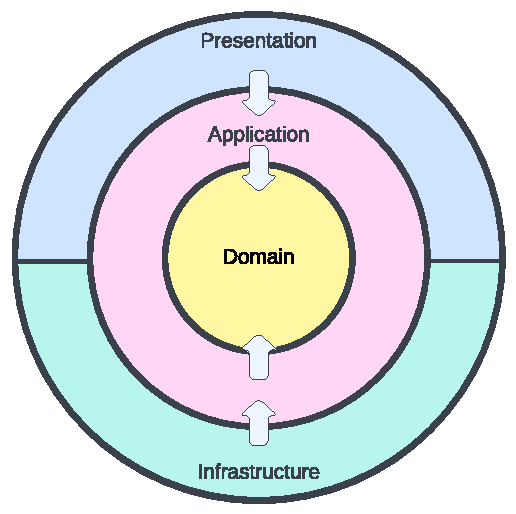
\includegraphics[width=0.4\textwidth]{Figures/ca_diagram.pdf}
    \caption[modularity]{Flow of control}
    \label{fig_modulair_components}
\end{figure}